\documentclass[../main.tex]{subfiles}

\begin{document}

\section{La vulnerabilidad \it{Log4shell}}

\it{Log4Shell} es el nombre que se le ha dado a la vulnerabilidad \it{CVE-2021-44228} \cite{cve-log4shell}, descubierta en la biblioteca \it{Log4J} por \it{Alibaba Cloud} el 24 de noviembre de 2021, y que fue hecha pública por la fundación \it{Apache} el 9 de diciembre de ese mismo año \cite{log4j-vulnerabilities}.

Se trata de una vulnerabilidad crítica, pues permite la ejecución de código arbitrario en cualquier sistema que use una versión de \it{Log4J} comprometida para registrar eventos. Algunos medios, de hecho, la han catalogado como la vulnerabilidad más crítica de la última década \cite{log4shell-noticia}, esto debido a la gravedad que tiene y la facilidad de su explotación.

La vulnerabilidad, como tal, consiste en la sustitución de las macros \it{jndi} de manera incontrolada, de forma que se permite que cualquier clase ubicada remotamente sea cargada y ejecutada en la máquina que ejecuta \it{Log4j} para registrar su traza, al nivel de privilegios con el que esa aplicación se esté ejecutando.

%--------------------------------------------------
\subsection{Localización en los fuentes}

El problema se debe a que la implementación original del soporte al API \it{JNDI} se hizo de forma que no se aplicaba ninguna restricción acerca de qué nombres podían resolverse, por lo que el uso de algunos protocolos, como \it{LDAP}, no es seguro en esas versiones de \it{Log4J} al permitir la ejecución remota de código.

Como tal, el fragmento de código causante de la brecha de seguridad es el método \it{lookup} de la clase \it{jndiManager}, tal y como afirman algunos análisis \cite{log4shell-cause-sophos}.

La versión \it{2.15.0} corrigió en parte el problema al restringir el API \it{JNDI} a búsquedas mediante \it{LDAP}, y limitar éstas últimas a búsquedas de objetos en el propio host de forma predeterminada. No obstante, esto no solucionó del todo el problema, por lo que apareció una segunda vulnerabilidad \it{Log4Shell} \cite{cve-log4shell-2}, que en este caso se puede explotar para perpetrar ataques de denegación de servicio. Finalmente, este fallo también se corrigió en la versión \it{2.17.0}, que se puede considerar la primera totalmente parcheada.

Lo que resta del trabajo se centrará solo en la primera vulnerabilidad \it{Log4Shell}, pues es la más crítica y la que mayor impacto ha tenido.

%--------------------------------------------------
\subsection{Detección}

Desde que se tiene constancia de ello, se han desarrollado diversos scanners que permiten buscar la vulnerabilidad dada una URL o directamente inspeccionando ficheros con bytecode.

Para detectar si un servidor web presenta la vulnerabilidad se ha utilizado el proyecto de GitHub de la agencia de seguridad de Estados Unidos, desarrollado para detectar \it{Log4Shell} \cite{scanner-cisagov}. La parte de éste que se va a utilizar (directorio \it{log4j-scanner}), no obstante, se basa en realidad en este otro proyecto \cite{scanner-cisagov-original}.

Su funcionamiento es el siguiente; el script \it{log4j-scan.py} envía peticiones al servidor web indicado introduciendo \it{lookups} de \it{Log4J} de manera sistemática en cada uno de los campos de la cabecera HTTP que se hayan especificado en el fichero \it{headers.txt}. Estas macros, en caso de ser interpretadas por una versión vulnerable de \it{Log4J}, cargarán una clase Java a modo de canario que le enviará un callback al script, de forma que éste podrá detectar si el servidor web se ha visto comprometido.

Con los siguientes comandos se clona el repositorio y se instalan las dependencias necesarias para las pruebas que se van a realizar:
\begin{codigo}{shell}
# Clonar repositorio
git clone https://github.com/cisagov/log4j-scanner.git
# Instalar dependencias de Python
cd log4j-scanner/log4j-scanner/
pip3 install -r requirements.txt
\end{codigo}

Después, suponiendo que el servidor web que se desea inspeccionar tiene como dirección \it{192.168.56.200} y puerto \it{8080}, el scanning consiste en ejecutar el script \it{log4j-scan.py} con los argumentos siguientes:
\begin{codigo}{shell}
./log4j-scan.py -u http://192.168.56.200:8080
\end{codigo}

El resultado de su ejecución se muestra en la siguiente captura de pantalla:
\begin{figure}[!h]
\centering
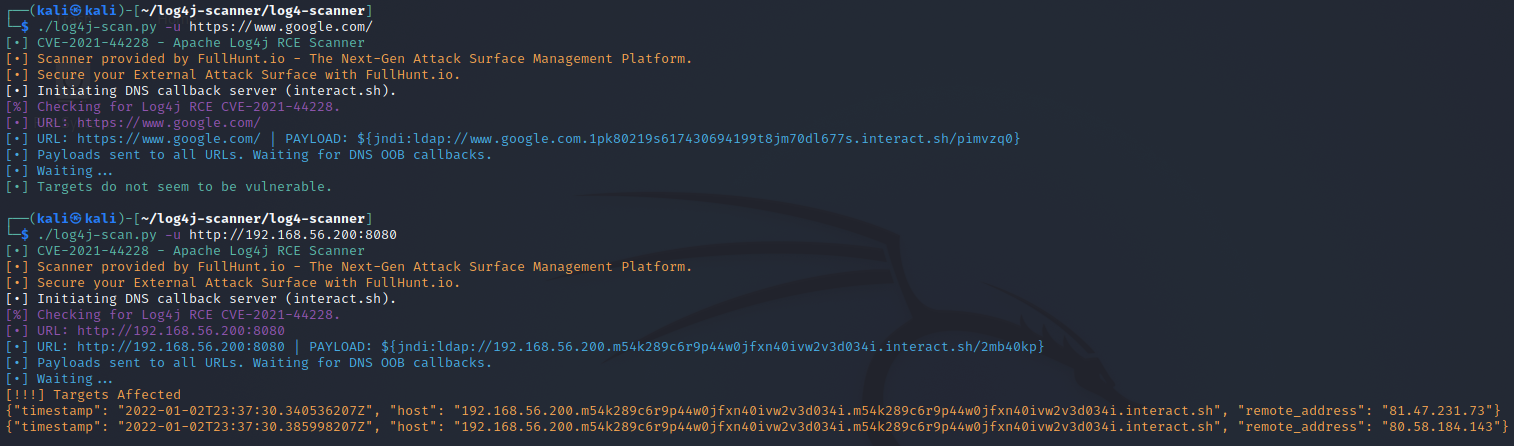
\includegraphics[width=15.0cm]{imagenes/2-Log4Shell/scanner_no-vulnerable-vs-vulnerable.png}
\caption{Resultados de la ejecución del script 'log4j-scan.py': arriba, para un servidor web que no es vulnerable a Log4Shell, abajo, para un servidor que sí es vulnerable}
\end{figure}

Se puede ver como en el caso de \it{google.com}, el scanner no ha detectado ningún objetivo (entendido como campo de la cabecera HTTP) vulnerable, mientras que en la aplicación web vulnerable \cite{vulnerable-app} lanzada en una máquina virtual sí (concretamente en dos de ellos).

\end{document}